\documentclass[openany, 10pt]{article}
\usepackage[a4paper,margin=1in]{geometry} % Adjust margins as needed
\usepackage{enumitem}
\usepackage{listings}
\usepackage{hyperref}
\usepackage{tikz}
\usepackage{xcolor}
\usepackage{biblatex}
\addbibresource{Physically_Based_Rendering_fourth_editio.bibtex}

\usetikzlibrary{shapes.geometric, arrows, positioning, fit}

\tikzstyle{startstop} = [rectangle, rounded corners, minimum width=3cm, minimum height=1cm,text centered, draw=black, fill=red!30]
\tikzstyle{process} = [rectangle, minimum width=3cm, minimum height=1cm, text centered, draw=black, fill=blue!30]
\tikzstyle{subprocess} = [rectangle, minimum width=3cm, minimum height=1cm, text centered, draw=black, fill=green!30]
\tikzstyle{arrow} = [thick,->,>=stealth]
\tikzstyle{stage} = [text centered, draw=black, dashed, inner sep=0.5cm]

\begin{document}
\begin{center}
    {\Huge \textbf{Project Proposal}} \\[2em]
\end{center}
\begin{flushright}
    \textbf{Tanzi Alessio} \\
    \textbf{Di Gregorio Antonino}
\end{flushright}
\section{Project}
Path tracing, a cornerstone algorithm in physically based rendering, provides realistic image synthesis by simulating the complex interactions of light. 
However, its computational demands make necessitate efficient implementations. This proposal explores a \textit{wavefront-based} approach to optimize the path tracing algorithm 
using NVIDIA's CUDA framework, leveraging GPU parallelism to maximize throughput and minimize latency. \par
Unlike traditional monolithic kernel implementations, the wavefront approach\cite{pharr2023physically} decomposes path tracing into distinct stages, such as ray generation, 
intersection testing, shading, and path termination. \par 
Each stage operates as an independent kernel, allowing for reduced divergence across threads. It is possible to combine such a pipeline structure with the concept of 
\textit{packet tracing}, meaning processing multiple spatially coherent rays in parallel. The project aims to exploit CUDA's features, such as shared memory, and streams, 
to efficiently manage these wavefront stages while addressing synchronization challenges inherent in multi-kernel workflows. \par
By implementing and benchmarking this wavefront path tracing system, the project seeks to explore the aforementioned implementation and measure it terms of render time to 
reach a given variance, and comparing these to exising rendering systems like \textit{PBRT-v4} and \textit{MoonRay}.\par
% Inserire gli ultimi avanzi per l'algoritmo di path tracing, quindi rendering spettrale, quindi geatione bidirezionale della luce, 
% quindi metropolis hastings
Our GPU implementation will use \href{https://raytracing-docs.nvidia.com/optix8/guide/index.html}{NVIDIA OptiX}, while our CPU based implementation will use
\href{https://github.com/RenderKit/embree}{Embree}
\section{Theory Overview}
The algorithm describes the process of rendering an image, starting with the Camera Model. This model generates camera rays, sets sample times, culls out-of-view objects,
 and computes depth of field using a Gaussian lens. Depth of field is achieved by sampling a point on the lens, shooting two rays, and averaging their radiance contributions. 
 Rays propagate through the scene, carrying radiance along their inverse paths, ultimately forming a grid of radiance samples on the image plane (the "film").

The Sensor Model processes this grid, computing RGB responses using spectral power distributions (SPDs) and applying white balancing via the von Kries Transform. 
The resulting irradiance grid is aggregated into pixel values using a weighted average based on Monte Carlo sampling probability. 
The Sampler, using methods like the Halton sequence, determines sample placement on the film, and a Reconstruction Filter (e.g., Mitchell-Netravali) 
processes the irradiance responses, emphasizing image details.

During ray propagation, the algorithm assumes void space, focusing on ray interactions and surface reflection. Scenes are partitioned into Bounding Volume Hierarchies (BVH) 
to optimize intersection tests. When a ray intersects a surface, reflection is modeled using BRDFs/BTDFs, often leveraging Microfacet Theory. This theory treats surfaces as 
collections of micro-planes, applying Snell's Law, Fresnel equations, and shadowing/masking factors to compute reflectance and transmittance. Models like Torrance-Sparrow 
use parameters like color, roughness, and metallicity, which can be texture-mapped.

\section{Brief of the Algorithm}
\begin{figure}[t]
  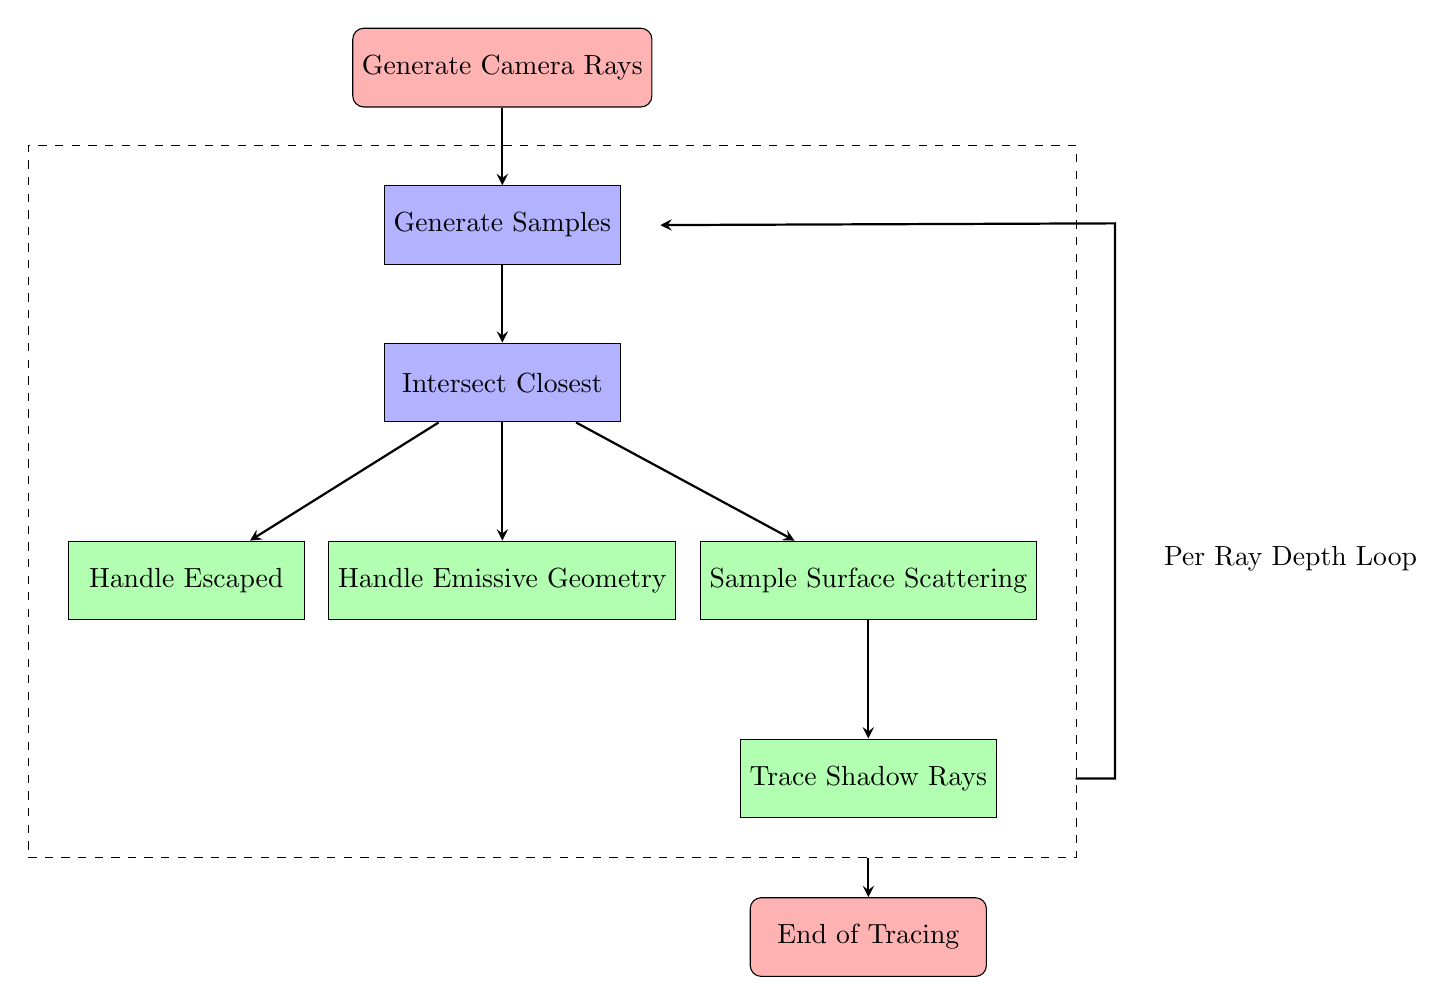
\begin{tikzpicture}[node distance=1.5cm]
  % Nodes for main flow
  \node (start) [startstop] {Generate Camera Rays};
  \node (generate) [process, below of=start, yshift=-0.5cm] {Generate Samples};
  \node (intersect) [process, below of=generate, yshift=-0.5cm] {Intersect Closest};

  % Sub-process nodes for Intersect Closest
  \node (escaped) [subprocess, below left=1.5cm and 1cm of intersect] {Handle Escaped};
  \node (emissive) [subprocess, below=1.5cm of intersect] {Handle Emissive Geometry};
  \node (scattering) [subprocess, below right=1.5cm and 1cm of intersect] {Sample Surface Scattering};

  % Sub-process for Sample Surface Scattering
  \node (shadow) [subprocess, below=1.5cm of scattering] {Trace Shadow Rays};

  % Loops for depth
  \node (loopstart) [stage, fit={(generate) (shadow) (intersect) (escaped) (emissive) (scattering)}] {};

  % Loops for depth (right label)
  \node (looplabel) [above right=2.0cm and 2.0cm of shadow] {Per Ray Depth Loop};

  % End
  \node (end) [startstop, below=1cm of shadow] {End of Tracing};

  % Arrows for main flow
  \draw [arrow] (start) -- (generate);
  \draw [arrow] (generate) -- (intersect);

  % Arrows to sub-processes
  \draw [arrow] (intersect) -- (escaped);
  \draw [arrow] (intersect) -- (emissive);
  \draw [arrow] (intersect) -- (scattering);

  \draw [arrow] (scattering) -- (shadow);

  % Loop back to start of depth
  \draw [arrow] (shadow.east) ++(1,0) -- ++(0.5,0) -- ++(0, 7.05) -- ([xshift=0.5cm]generate.east);

  % Arrow to end
  \draw [arrow] (shadow.south) ++(0,-0.5) -- ++(0,-0.3) -- (end.north);

  \end{tikzpicture}
  \caption{Diagram showing kernel execution for a GPU path tracer with the wavefront architecture}
  \label{gif}
\end{figure}

While in a typical CPU implementation, introducing multiprocessing is done through decomposition of the image in tiles and let each core process a packet of rays generated 
inside each with the use of SIMD instruction, such an approach in the GPU is fundamentally flawed by the fact that there aren't nearly enough tiles in a typical high resolution
image to prepare enough workloads to achieve a sufficient GPU hardware utilization. Hence there are fundamentally two approaches to a GPU Path tracer, detailed below:
% labelwidth area riservata a labels, labelsep separazione tralabel e testo, leftmargin il margine
\begin{itemize}[topsep=0pt, noitemsep, labelwidth=3cm, labelsep=1em, leftmargin=4cm] 
  \item[\textbf{megakernel}] assign each pixel sample to a thread, and execute a kernel which handles the whole path tracing algorithm. Since Rays will hit different spatial 
    positions, it is reasonable that the major problem for this approach is \texttt{Divergence}, which can be mitigated by organizing Queues of coherent work units, executed by 
    each warp. Even with this, the other disadvantage of such approach is that the code amout of the kernel is huge. Furthermore, even with job scheduling, it is impossible to 
    completely eliminate divergence
  \item[\textbf{wavefront}] Separate the main operations into different kernels. This allows to allocate less registers to simpler kernels and to handle the complexity and 
    convergence problems which arise from the megakernel approach. Nevertheless, they pay the price for such additional flexibility in memory traffic, since the only way kernels
    have to communicate is through Global Memory\footnote{we are assuming rendering over a single GPU}
\end{itemize}
We will follow the latter approach, hence having
\begin{itemize}[topsep=0pt, noitemsep]
  \item A first kernel generating camera samples and keeping them in device memory for later use
  \item find closest interaction and store intersection information in 3 different queues, one for escaped rays, one for rays that hit a light, and one for
    rays that hit a surface
  \item the kernels of escaped rays and of rays which hit an emissive geometry are responsible to update radiance estimation over the path traced by therr rays 
  \item the kernels which handle each type of surface are responsible to compute transmittance and reflectance factors, and enqueue indirect rays and shadow rays respectively
    for the shadow rays step and the next iteration
  \item most of the kernels, as mentioned above, generate some indirect rays which need to be traced again, therefore the specified kernels are launched again a number of times
    specified by the maximum depth (or bounces) for the algorithm, as shown in Figure \ref{gif}
\end{itemize}
Final Notes:
\begin{itemize}[topsep=0pt, noitemsep]
  \item Emphasis is drawn to the memory layout of each of the object (eg. surface interaction information, ray data), which in typical implementation are 
    stored in a Structure of Arrays layout
  \item The scenes will be stored in the \texttt{.pbrt} format, for which scenes are already available in this \href{https://github.com/mmp/pbrt-v4-scenes}{GitHub Link},
    and a parser is available on the \href{https://github.com/mmp/pbrt-v4}{PBRT-v4 Repository}
  \item The loop for kernel execution is made on the CPU over \textit{Wavefront Depth}. One possible approach is to ignore the state of execution of the algorithm, meaning 
    that the CPU will still launch the kernels up to max depth, even if all rays escape the scene after the first intersection test
\end{itemize}

% inserire le due fondamentali famiglie di architetture, cioe il megakernel e wavefront. andremo con il wavefront, un po perche 
% e quello che segue PBRT e un po perche e quello che implementano in hardware i RT cores delle GPU moderne
% 
% Useremo compute capability cc6.0 perche ho una gtx 1070, quindi no thread independent scheduling, no cooperative groups.
% Dire cosa deve fare ogni kernel e che tipo di sincronizzazione ci deve essere, quindi se si utilizzamo le streams o i graphs, 
% se lo possiamo fare lo schema si presta bene con i grafi
% dettagliare il memory layout e quindi come gestire la shared memory
% 
% embree -> CPU ray tracing
% optiX  -> GPU ray tracing

% double buffering per streammare tutti i risultati alla cpu per evalugtare la varianza

\printbibliography

\end{document}
